\section{Hardware}

HW må lages slik at det støtter innhenting og utsending av data fra to vibrasjonssensorer. 
For å samle og sende data trengs en MCU, og for å kunne måle spenningsverdiene fra sensorene
må denne MCUen ha minst to ADC kanaler. Hver sensor kobles til hver sin ADC kanal, eventuelt
med en forsterkerkrets mellom sensor og MCU dersom nødvendig å forsterke signalet.
Avhengig av frekvensen på signalene som skal fanges og ønsket samplingsrate av signalet, må 
MCUen ha en ADC som støtter ønsket samplinger per sekund. I tillegg må HW sende dataen 
videre til kontrollsystemet for videre analyse. For å koble sammen HW og SW som analyserer data,
må det eksistere et nettverk mellom HW og SW. Det mest praktiske og enkleste er å ta i bruk det eksisterende
nettverket som allerede er installert i lastebiler. Da må HW støtte CAN bus protokollen enten innebygget
i MCUen eller som en egen integrertkrets. Begge alternativer er gode, men kostnad vil nok favorisere
én mindre integrert krets. Firmaren \cite{firmware} som skal ligge i minnet på MCUen krever lite plass, 
da dette innvevde systemet \cite{embedded} kun skal ligge i dvale til det skal ta en lydprøve og sende 
videre. Dagens MCUer kommer i mange
ulike varianter, så å finne en MCU som har god nok oppløsning på ADC og kan kommunisere over CAN
er ikke noe problem. 

Fordelen med denne løsningen er at man får sentralisert analysering av lydprøver i kontrollenheten.
Det gir mulighet for raskere endring av software og erfaringsbasert analyse. Det reduserer også kompleksiteten
av HW som igjen fører til redusert kost. 

Figur \ref{fig:hw} viser en prototype som støtter sensorer og har riktig nettverkstilkoblinger. 
\begin{figure}[H] \centering
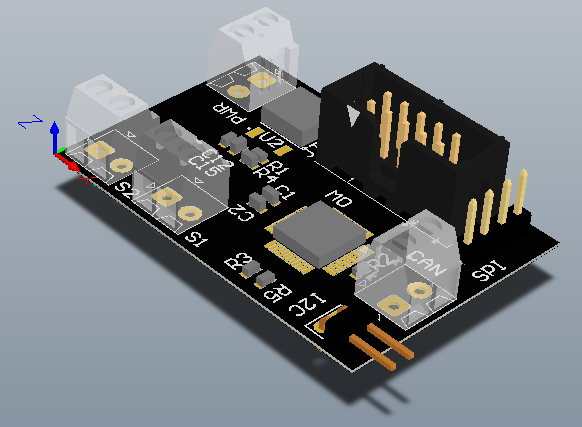
\includegraphics[width=0.5 \textwidth]{images/eit_prototype.png}
\caption{Prototype av hardware module.}
\label{fig:hw}
\end{figure}
Løsningen baserer seg på at analysen skjer i SW og at HW er så enkel som mulig. Dette gir mer
fleksibilitet med tanke på oppdateringer og utvidelse av bruksområder i analysen.